\chapter{Descrizione del Progetto}
\label{cap:descrizione}

\textit{\indent Questo capitolo fornisce il background tecnico essenziale per comprendere il progetto, analizza le problematiche delle tecnologie coinvolte e illustra l'idea fondamentale alla base del lavoro svolto.}

\section{Background}

~\\
\indent Questa sezione illustra il funzionamento e i principi fondamentali delle tecnologie chiave del progetto.
Quest'ultime costituiscono la base essenziale per la comprensione di questo studio. 

\subsection{Protocolli di Trasporto Tradizionali}
~\\
\indent Nel panorama dei \emph{protocolli di rete}\footnote{\gls{protocolli di rete}}, i \emph{protocolli di trasporto}\footnote{\gls{protocolli di trasporto}} \emph{TCP (Transmission Control Protocol)}  e \emph{UDP (User Datagram Protocol)} hanno svolto e svolgono tutt'ora un ruolo fondamentale sin dalla nascita di Internet.
Questi protocolli sono stati la spina dorsale delle comunicazioni per decenni, supportando una vasta gamma di servizi e applicazioni.\\
In particolare \emph{TCP}, con la sua affidabilità e il suo controllo di flusso, ha svolto un ruolo fondamentale nelle comunicazioni che richiedevano l'integrità dei dati, mentre \emph{UDP} ha trovato il suo spazio nei servizi che privilegiavano la velocità rispetto all'affidabilità. 
Tuttavia, con l'evoluzione delle nuove tecnologie, le limitazioni di questi protocolli sono diventate sempre più evidenti. Nella concezione di base di \emph{TCP} e \emph{UDP}, ideata agli inizi del 1970, non erano state previste le sfide delle reti moderne, 
caratterizzate da:  
\begin{itemize}
    \item Connesioni mobili e variabili;
    
    \item Necessità di ridurre la latenza;
    
    \item Proliferazione di dispositivi \emph{IoT}\footnote{\gls{IoT}};
     
    \item Requisiti di sicurezza sempre più vincolanti.
\end{itemize}

\noindent Queste nuove sfide hanno evidenziato una serie di problematiche nei protocolli. La consapevolezza di questi limiti ha portato alla ricerca di nuove soluzioni, cercando di superare le inefficienze pur mantenendo tutti i punti di forza.
Questi studi hanno portato alla creazione di nuovi protocolli come \emph{QUIC} ed a estensioni come \emph{MPTCP}, che cercano di far fronte alle sfide del mondo moderno offrendo prestazioni migliori, maggiore sicurezza e flessibilità.
\\
\\
Nelle sezioni successive esamineremo in dettaglio alcune parti di \emph{TCP} e \emph{UDP}, per poi esplorare come \emph{QUIC} e \emph{MPTCP} si propongono di risolvere e superare le inefficienze presenti e le possibili ripercussioni.

\subsubsection{TCP (Transmission Control Protocol)}
~\\
% Fonte https://www.ietf.org/rfc/rfc793.txt %
\indent Il \emph{Transmission Control Protocol (TCP)}, come anticipato nella sezione precedente, è uno dei protocolli cardine su cui si basa la comunicazione su Internet. Dato il suo ruolo e la vasta gamma di funzioni che offre, un'analisi completa del suo funzionamento e della sua costituzione richiederebbe un'analisi approfondità che va oltre lo scopo di questa tesi. Pertanto, in questa sezione, ci concentreremo solo su alcuni aspetti specifici del \emph{TCP} che sono fondamentali per la comprensione del nostro studio su \emph{QUIC}. 
In particolare, esamineremo nel dettaglio :
\begin{itemize}
    \item Caratteristiche principali di una connessione \emph{TCP};
    
    \item Il processo di \emph{Handshake}\footnote{\gls{Handshake}};
    
    \item Il meccanismo di Ritrasmissione;
    
    \item I metodi utilizzati per garantire la sicurezza dei dati.
\end{itemize}

\paragraph{\textit{Caratteristiche principali}}
\noindent Il \emph{Transmission Control Protocol} si distingue come un protocollo orientato alla connessione. Questa sua caratteristica significa che, prima di qualsiasi scambio di dati, deve essere stabilita una connessione dedicata tra il \emph{client}\footnote{\gls{client}} e il \emph{server}\footnote{\gls{server}}.
Questa peculiarità è alla base di molte delle sue funzionalità avanzate, tra cui:
\begin{description}
    \item[Affidabilità] Viene utilizzato il meccanismo degli \emph{acknowledgement}\footnote{\gls{acknowledgements}} per garantire la corretta consegna dei segmenti.

    \item[Controllo di Errore] Implementa un sistema di verifica della integrità dei dati tramite il meccanismo degli \emph{checksum}\footnote{\gls{checksum}}.
    
    \item[Controllo di Flusso e Congestione] Utilizza il sistema delle \emph{sliding window}\footnote{\gls{sliding window}} per ottimizzare il flusso di dati e diminuire il numero di segmenti ritrasmessi in caso di situazione di congestione.
\end{description}

\noindent Queste funzionalità si riflettono sulla struttura stessa di un segmento \emph{TCP}, come si può vedere nella Figura \ref{fig}. Segue una breve descrizione di alcune delle sezioni a noi necessarie:

\begin{itemize}
\item \textit{\textbf{Source Port - Destination Port}}: Identificano rispettivamente il numero della porta di origine e destinazione.
\item \textit{\textbf{Sequence Number}}: Definisce il \emph{sequence number}, che indica la posizione del primo segmento \emph{TCP} all'intenro del flusso. Inoltre se il \emph{control bits SYN} è presente allora il \emph{sequence number} rappresenta il \emph{ISN}\footnote{\gls{ISN}} e il primo otteto successivo avrà come \emph{sequence number ISN+1}.
\item \textit{\textbf{Acknowledgement Number}}: Se il \emph{control bits ACK} è presente questo campo contiene il valore del prossimo \emph{sequence number} che il ricevente del segmento si aspetta di ricevere.
\item \textit{\textbf{Control Bits}}: Sono dei bit utilizzati per il controllo del protocollo. 
\begin{itemize}
    \item \textit{\textbf{URG}}: Se impostato a 1 indica la presenza di dati urgenti.
    \item \textit{\textbf{ACK}}: Se impostato a 1 indica che l'\emph{acknowledgement number} è valido.
    \item \textit{\textbf{PSH}}: Se impostato a 1 indica che i dati devono essere elaborati dai livelli superiori.
    \item \textit{\textbf{RST}}: Se impostato a 1 indica che la connesione non è più valida.
    \item \textit{\textbf{SYN}}: Se impostato a 1 indica che il mittente vuole stabilire una connesione \emph{TCP}.
    \item \textit{\textbf{FIN}}: Se impostato a 1 indica che il mittente vuole terminare la connessione \emph{TCP}.
\end{itemize}
\item \textit{\textbf{Checksum}}: Valore utilizzato per verificare la validità del segmento. Si ottiene facendo il complemento a uno della somma complementare a uno a 16 bit dell'\emph{header}, del \emph{payload} e altri di valori.
\item \textit{\textbf{Data}}: Rappresenta il vero e proprio \emph{payload} da trasmettere.
\end{itemize}

\begin{figure}[!h]
\centering
\begin{BVerbatim}
 0                   1                   2                   3   
 0 1 2 3 4 5 6 7 8 9 0 1 2 3 4 5 6 7 8 9 0 1 2 3 4 5 6 7 8 9 0 1 
+-+-+-+-+-+-+-+-+-+-+-+-+-+-+-+-+-+-+-+-+-+-+-+-+-+-+-+-+-+-+-+-+
|          Source Port          |       Destination Port        |
+-+-+-+-+-+-+-+-+-+-+-+-+-+-+-+-+-+-+-+-+-+-+-+-+-+-+-+-+-+-+-+-+
|                        Sequence Number                        |
+-+-+-+-+-+-+-+-+-+-+-+-+-+-+-+-+-+-+-+-+-+-+-+-+-+-+-+-+-+-+-+-+
|                    Acknowledgment Number                      |
+-+-+-+-+-+-+-+-+-+-+-+-+-+-+-+-+-+-+-+-+-+-+-+-+-+-+-+-+-+-+-+-+
|  Data |           |U|A|P|R|S|F|                               |
| Offset| Reserved  |R|C|S|S|Y|I|            Window             |
|       |           |G|K|H|T|N|N|                               |
+-+-+-+-+-+-+-+-+-+-+-+-+-+-+-+-+-+-+-+-+-+-+-+-+-+-+-+-+-+-+-+-+
|           Checksum            |         Urgent Pointer        |
+-+-+-+-+-+-+-+-+-+-+-+-+-+-+-+-+-+-+-+-+-+-+-+-+-+-+-+-+-+-+-+-+
|                    Options                    |    Padding    |
+-+-+-+-+-+-+-+-+-+-+-+-+-+-+-+-+-+-+-+-+-+-+-+-+-+-+-+-+-+-+-+-+
|                             data                              |
+-+-+-+-+-+-+-+-+-+-+-+-+-+-+-+-+-+-+-+-+-+-+-+-+-+-+-+-+-+-+-+-+
           \end{BVerbatim}
\caption{Segmento TCP}
\label{fig}
\end{figure}

\noindent È importante quindi notare che per costruzione il protocollo identifica univocamente una connesione \emph{TCP} con una tupla composta da 4 elementi:

\begin{center}
    \small
    $[\text{Indirizzo IP sorgente}, \text{Porta sorgente}] \leftrightarrow [\text{Indirizzo IP destinazione}, \text{Porta destinazione}]$
\end{center}

\noindent Questa struttura offre diversi vantaggi. Permettere a un singolo \emph{server} di accettare più connessioni contemporaneamente da diversi \emph{client}, e viceversa. 
Inoltre garantisce l'unicità di ogni connessione all'interno della rete.
\\
Tuttavia, questa rigida definzione comporta delle limitazioni significative. In quanto una qualsiasi modifica ad un elemento della tupla (ad esempio, un cambiamento di porta o una migrazione dell'indirizzo IP) comporta la terminazione della connesione esistente. Questo diventa ancora più limitativo nel contesto delle comunicazioni moderne dove i casi di \emph{multihoming}\footnote{\gls{multihoming}} e cambi frequenti di indirizzo IP sono sempre più comuni.
\\
\\
Questa problematica, come vedremo nelle prossime sezioni, è alla base di soluzioni come \emph{MPTCP} e viene affrontata in modo indiretto anche in \emph{QUIC}.

\paragraph{\textit{Handshake}}
% https://it.wikipedia.org/wiki/Round_Trip_Time

\noindent Come accennato in precedenza, uno dei punti cardine del \emph{TCP} è la necessità di stabilire una connessione prima di qualsiasi scambio di dati. Questo processo, noto come \emph{three-way handshake} ("stretta di mano in tre passaggi"), richiede lo scambio di tre messaggi tra \emph{server} e \emph{client}. La Figura \ref{handshake} illustra questo processo.

\begin{figure}[!h]
    \centering
    \begin{minipage}{0.48\textwidth}
        \centering
        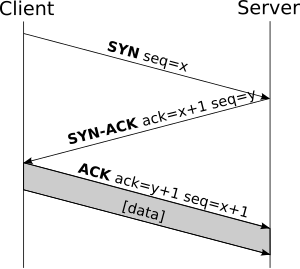
\includegraphics[width=0.75\columnwidth]{descrizione/tcp/three-way-handshake}
        \caption{\emph{three-way handshake}}
        \label{handshake}
    \end{minipage}
    \hfill
    \begin{minipage}{0.48\textwidth}
        \centering
        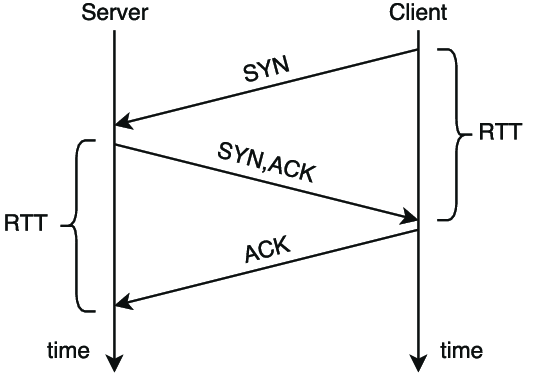
\includegraphics[width=0.90\columnwidth]{descrizione/tcp/rtt-handshake}
        \caption{\emph{RTT (Round Trip Time)}}
        \label{rtt}
    \end{minipage}
\end{figure}

\noindent Segue ora una breve spiegazione dei passaggi che avvengono in questo processo : 

\begin{enumerate}
    \item \textbf{Client invia un segmento SYN al Server}: Il segmento ha il campo \emph{SYN} impostato a 1 e il suo \emph{sequence number} contiene il \emph{ISN (Initial Sequence Number)} del Client.
    \item \textbf{Server invia un segmento SYN/ACK al Client}: Il Server risponde con un segmento i cui campi \emph{SYN} e \emph{ACK} sono impostati a 1. Il suo \emph{sequence number} contiene un nuovo valore y mentre l'\emph{Acknowledgement number} contiene il valore \emph{ISN+1}.
    \item \textbf{Client invia un segmento ACK al Server}: Il Client risponde inviando un segmento il cui campo \emph{ACK} è impostato a 1 e l'\emph{acknowledgement number} è dato da \emph{y+1}.
\end{enumerate}

\noindent Tutti i segmenti utilizzati in questa fase hanno il campo \emph{data} vuoto, ossia sono solamente degli \emph{header}. 
Oltre a stabilire la connessione, l'\emph{handshake} riveste un ruolo fondamentale in vari aspetti della comunicazione \emph{TCP}.
Non solo permette di sincronizzare i \emph{sequence number}, ma fornisce anche una base inziale per misurare il \emph{RTT}\footnote{\gls{RTT}} (Figura \ref{rtt}), che è essenziale per ottimizzare il controllo di flusso e la gestione della congestione della rete.

\paragraph{\textit{Ritrasmissioni}}

\noindent La gestione degli errori nel \emph{TCP} è un argomento estremamente complesso che necessiterebbe di uno studio dedicato. 
Tuttavia, ciò va oltre allo scopo di questa tesi e per motivi di spazio non verrà discusso. Pertanto ci limiteremo a descrivere brevemente il meccanismo di ritrasmissione, necessario per comprendere alcuni concetti della tesi.
\\\\
\noindent Il \emph{TCP} è un protocollo progettato per garantire l'affidabilità nella trasmissione dei dati. La ritrasmissione dei segmenti persi o danneggiati è uno dei meccanismi chiave per raggiungere questo obbiettivo. Questo processo si basa sulla logica degli \emph{acknowledgements}. Quando un segmento viene inviato, il mittente attende una conferma di ricezione (\emph{ACK}) dal destinatario. Se questa conferma non viene ricevuta entro un determinato intervallo di tempo, chiamato \emph{RTO}\footnote{\gls{RTO}}, il mittente assume che il segmento sia stato perso e lo ritrasmette.
In particolare, è importante sapere che il calcolo del RTO è dinamico e dipende fortemente dal \emph{RTT} e da numerosi altri valori. 
\\\\
\noindent(Si puo' dedicare piu' spazio a questa sezione approndendo casistiche e meccanismi ulteriori)
\\\\
\noindent(Forse fuori tema e da rimuovere)(inerente nel caso si testasse sulle reti mobili)
\\
Sono numerose le cause che possono provocare la perdita di un pacchetto. Nel caso delle reti mobile ciò può accadere in punti diversi dell'infrasstruttura. Nel caso il segmento venga perso tra il client e la stazione base in \emph{RAN}\footnote{\gls{RAN}} è compito del \emph{link layer} occuparsi della ritrasmissione. Questo significa che, se il pacchetto venisse perso un numero di volte ma poi venisse ricevuto, il \emph{TCP} non rileverebbe alcun pacchetto perso ma solo un aumento del \emph{RTT}.
\paragraph{\textit{Sicurezza}}

\noindent Nella sua forma nativa, il protocollo \emph{TCP}, non offre meccanismi di sicurezza come autenticazione, integrità dei dati o confidenzialità. Infatti, \emph{TCP} non implementa alcuna funzionalità di crittografia o altri sistemi con lo scopo di proteggere i dati durante la trasmissione.
Per colmare questa mancanza, vengono utlizzati protocolli aggiuntivi come il \emph{TLS}\footnote{\gls{TLS}} e il \emph{SSL}\footnote{\gls{SSL}} (suo predecessore). Questi protocolli crittografici operano al \emph{livello di presentazione}\footnote{\gls{livello di presentazione}} del modello \emph{ISO/OSI}\footnote{\gls{ISO/OSI}} e di conseguenza ad un livello superiore rispetto al \emph{TCP}.
Forniscono entrambi le funzionalità di sicurezza essenziali, garantendo una comunicazione protetta e affidabile.
\\\\
Nel contesto di questo studio, ci concentreremo in particolare sul protocollo \emph{TLS 1.3}, l'ultima versione di esso. Esamineremo brevemente la nuova procedura di handshake (Figura \ref{tlsHand}), essenziale per negoziare i parametri di sicurezza e stabilire una comunicazione cifrata.
\begin{figure}[!h]
    \centering
    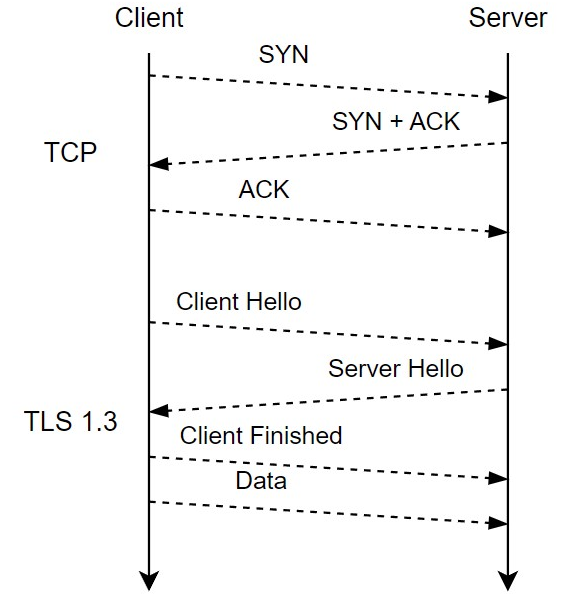
\includegraphics[width=0.7\columnwidth]{descrizione/tcp/tls-handshake}
    \caption{Nuovo Handshake (da modificare)}
    \label{tlsHand}
\end{figure}

\noindent Segue ora una breve spiegazione dei nuovi passaggi che avvengono in questo processo:
\begin{enumerate}
    \item \textbf{Client invia un messaggio ClientHello al Server}: Il messaggio contiene una lista dei cifrari supportati dal client;
    \item \textbf{Server risponde con un messaggio ServerHello al Client}: Il Server risponde con un messaggio che contiene: 
    \begin{itemize}
        \item  Il cifrario selezionato tra quelli inviati dal Client;
        \item  La chiave pubblica del server per l'algoritmo di scambio chiavi scelto.
    \end{itemize}
    Segue poi il messaggio \emph{Certificate}, che include il certificato del server, e un messaggio \emph{Finished} che conclude la sua parte dell'\emph{handshake};
    \item \textbf{Client invia un messaggio Finished}: Il Client dopo aver ricevuto il messaggio \emph{Finished} dal Server possiede tutte le informazioni necessarie per confermare il completamento dell'\emph{handshake} e invia a sua volta un messaggio \emph{Finished} per confermare il termine di tale operazione.
\end{enumerate}

\noindent È importante notare che con il \emph{TLS 1.3} si ha un \emph{2RTT}, ovvero vengono richiesti due \emph{Round Trip} prima dell'effettivo invio dei dati. 
\subsubsection{UDP (User Datagram Protocol)}
% https://datatracker.ietf.org/doc/html/rfc768
~\\
\indent Dopo aver esaminato brevemente il \emph{Transmission Control Protocol (TCP)},
procediamo ora all'analisi del \emph{User Datagram Protocol (UDP)}. 
Diversamente dal \emph{TCP}, questo protocollo si distingue per la sua semplicità e la minor complessità, offrendo un approccio più diretto alla trasmissione dei dati.
\\
Nonostante la sua relativa semplicità, una trattazione esaustiva dell'UDP andrebbe comunque oltre gli scopi di questa tesi. 
Di conseguenza ci concentreremo sulla struttura di un \emph{datagramma {UDP}} descritto in Figura \ref{udp-datagram}.
\\
\begin{figure}[!h]
    \centering
    \begin{BVerbatim}
 0      7 8     15 16    23 24    31
+--------+--------+--------+--------+
|     Source      |   Destination   |
|      Port       |      Port       |
+--------+--------+--------+--------+
|                 |                 |
|     Length      |    Checksum     |
+--------+--------+--------+--------+
|
|          data octets ...
+---------------- ...
        \end{BVerbatim}
    \caption{Datagramma UDP}
    \label{udp-datagram}
\end{figure}

\noindent Si può facilmente notare che l'\emph{header} di un datagramma \emph{UDP} è notevolmente più semplice rispetto a quello di un segmento \emph{TCP}.
In quanto questo è composto da soli quattro campi, i quali sono :  
\begin{itemize}
    \item \textit{\textbf{Source Port - Destination Port}}: Identificano rispettivamente il numero della porta di origine e destinazione. In questo caso il campo relativo alla \emph{source port} può essere omesso ed in tal caso settato a 0.
    \item \textit{\textbf{Lenght}}: Questo campo specifica la lunghezza in byte dell'\emph{header} e del \emph{payload}. La lunghezza minima è di 8 \emph{bytes} mentre il limite superiore è di 65,607 \emph{bytes}.
    \item \textit{\textbf{Checksum}}: Questo campo è opzionale e può essere usato per effettuare dei controli di errore sul datagramma.
\end{itemize}

\noindent La semplicità di questa struttura riflette a pieno i suoi casi d'uso, dove i punti di forza principali sono la velocità e l'efficienza.
In particolare l'assenza di complessi meccanismi di controllo e gestione, invece presenti nel \emph{TCP}, rende l'\emph{UDP} particolarmente adatto per applicazioni che richiedono una trasmissione rapida e in cui la perdita di alcuni pacchetti non invalida totalmente il servizio.
Ne sono un esempio i giochi online, lo streaming video e le chiamate \emph{VOIP}\footnote{\gls{VOIP}}.

\subsection{QUIC}
~\\
\indent Dopo aver esaminato brevemente alcuni dettagli dei protocolli di trasporto tradizionali (\emph{TCP} e \emph{UDP}), in questa sezione procederemo con l'analisi del protocollo argomento principale di questo studio. \\
Sviluppato inizialmente da \emph{Google} nel 2012, \emph{QUIC}\footnote{\gls{QUIC}} rappresenta un vero e proprio salto generazionale rispetto ai protocolli tradizionali, offrendo una soluzione che combina la velocità dell'\emph{UDP} alla sicurezza e affidabilità del \emph{TCP}. 
Il suo sviluppo così recente ha permesso di progettarlo specificamente per affrontare le sfide che i protocolli tradizionali faticavano a gestire, come le performance sulle reti mobili, la sicurezza e la latenza ridotta. Questo nuovo protocollo si è rapidamente affermato nel mondo delle comunicazioni, tanto da essere standardizzato dall'\emph{IETF}\footnote{\gls{IETF}} nel 2021.
\\\\
Inoltre \emph{QUIC} è stato progettato per collaborare con \emph{HTTP}\footnote{\gls{HTTP}}, il protocollo a \emph{livello applicativo}\footnote{\gls{livello applicativo}}. Chiamando \emph{HTTP/3}\footnote{\gls{HTTP/3}} la versione che utilizza \emph{QUIC} al posto di \emph{TCP} come protocollo di trasporto \cite{site:HTTP-over-QUIC}.
\\\\
\noindent Per motivi di spazio, analizzeremo solo gli elementi trattati durante il nostro studio, concentrandoci in particolare su questi argomenti:
\begin{itemize}
    \item La struttura del protocollo;
    \item Il processo di \emph{handshake};
    \item La gestione degli errori e le casistiche di Ritrasmissione;
    \item Sistemi di sicurezza;
    \item Versioni e Applicazioni;
\end{itemize}

\subsubsection{Struttura del Protocollo}
~\\ 
\indent Il protocollo \emph{QUIC}, come suggerisce il nome, è costruito sopra al protocollo \emph{UDP} per diversi motivi strategici. Questa scelta mira principalmente a evitare l'\emph{ossification}\footnote{\gls{ossification}}, un problema comune nello sviluppo di nuovi protocolli.
Questo perchè l'\emph{UDP} non solo è essenzialmente \emph{IP}(con l'aggiunta dei numeri di porta), ma anche perchè è ampiamente riconosciuto dalle \emph{middle box}\footnote{\gls{middle box}}, riducendo il rischio che un pacchetto \emph{QUIC} venga scartato.
Inoltre, \emph{UDP} non introduce alcun \emph{overhead}\footnote{\gls{overhead}} significativo e oltre a ciò è già integrato nei vari \emph{sistemi operativi}, cosa che non sarebbe vera se \emph{QUIC} si basasse direttamente su \emph{IP}.
\\
\begin{figure}[!h]
    \centering
    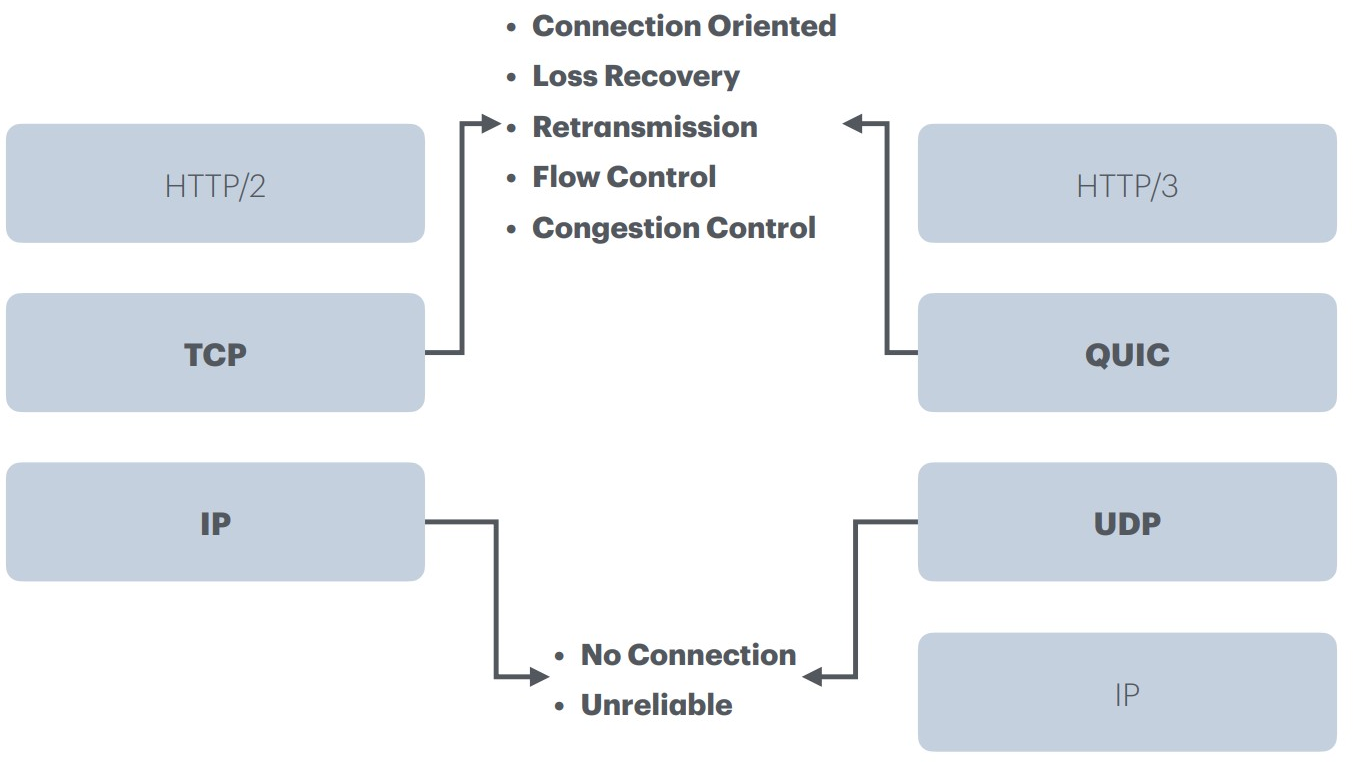
\includegraphics[width=0.7\columnwidth]{descrizione/quic/tcp-quic}
    \caption{\emph{TCP/IP - QUIC/UDP (da modificare)}}
    \label{tcp-quic}
\end{figure}

\noindent Come illutrato nella Figura \ref{tcp-quic} si può affermare che \emph{QUIC} si basa su \emph{UDP} in modo analogo a come \emph{TCP} si basa su \emph{IP}.
Nonostante questa differenza strutturale, \emph{QUIC} implementa le stesse funzionalità chiave di \emph{TCP}, seppur in modo diverso:
\begin{itemize}
    \item Orientato alla connessione;
    \item Recupero delle perdite;
    \item Controllo del flusso;
    \item Ritrasmissione;
    \item Controllo della congestione.
\end{itemize}

\noindent Un aspetto pratico importante è che, essendo costruito sopra \emph{UDP}, tutte le informazioni necessarie al funzionamento di \emph{QUIC} sono contenute nel payload del datagramma \emph{UDP} (Figura \ref{udp-datagram}).
\paragraph{\textit{Identificatori di Connessione}}
\noindent A differenza di \emph{TCP}, \emph{QUIC} adotta un approccio diverso e allo stesso tempo innovativo per l'identificazione delle connessioni. Mentre in \emph{TCP}, come abbiamo già visto, le connessioni sono identificate tramite la tupla:
\begin{center}
\small
$[\text{Indirizzo IP sorgente}, \text{Porta sorgente}] \leftrightarrow [\text{Indirizzo IP destinazione}, \text{Porta destinazione}]$
\end{center}
\emph{QUIC} introduce un concetto diverso: il \emph{Connection ID}\footnote{\gls{Connection ID}}. Questo identificatore consente di riconoscere la connessione in maniera indipendente dagli \emph{indirizzi IP} o dalle \emph{porte} utilizzate.
Il vantaggio principale di questo approccio è la capacità di mantenere attiva una connessione anche in caso di cambiamento dell'\emph{indirizzo IP} o della \emph{porta}, situazione che nelle reti moderne è molto frequente \cite{site:Explaining-QUIC}.
\\\\
Un esempio concreto che illustra gli effetti di questo approccio si può osservare nel comportamento dei dispositivi mobili durante il passaggio tra diverse reti.
Con una connessione \emph{TCP}, quando un dispositivo migra da una rete \emph{WiFi} a una \emph{rete mobile}, è richiesta una riconnessione completa (come si può vedere in Figura \ref{tcp-handoff}). 
\\
Al contrario,\emph{QUIC} gestisce questa transazione in modo più efficiente (come mostrato nella Figura \ref{quic-handoff}). Grazie al \emph{Connection ID}, \emph{QUIC} riesce a mantenere la connessione attiva nonostante il cambio di rete, eliminando la necessità di effettuare una riconnessione e garantendo un servizio costante.
\begin{figure}[!h]
    \centering
    \begin{minipage}{0.48\textwidth}
        \centering
        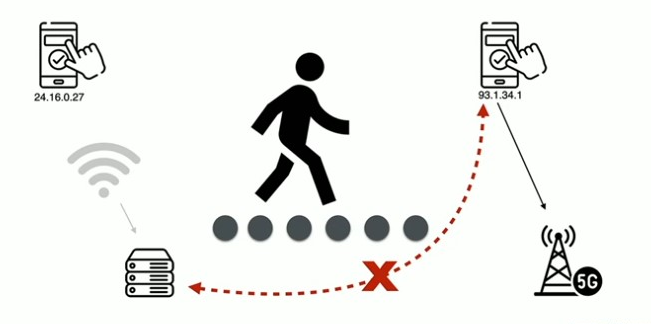
\includegraphics[width=0.90\columnwidth]{descrizione/quic/tcp-handoff}
        \caption{\emph{TCP}}
        \label{tcp-handoff}
    \end{minipage}
    \hfill
    \begin{minipage}{0.48\textwidth}
        \centering
        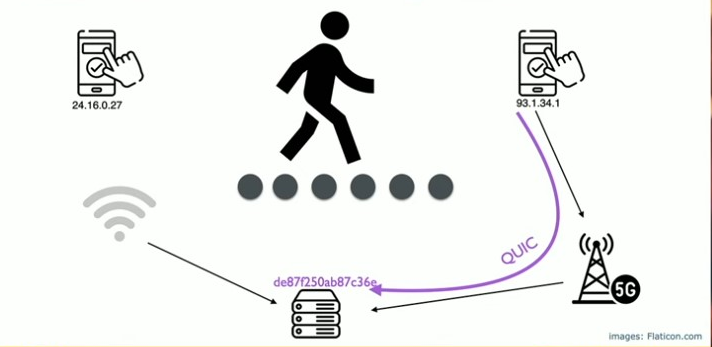
\includegraphics[width=0.90\columnwidth]{descrizione/quic/quic-handoff}
        \caption{\emph{QUIC}}
        \label{quic-handoff}
    \end{minipage}
\end{figure}
\\
Oltre a questo vantaggio fondamentale, l'utilizzo del \emph{Connection ID} offre ulteriori benefici:
\begin{itemize}
\item \textbf{Load balancing}: Grazie al \emph{Connection ID} i server possono distribuire il carico in modo più dinamico senza avere interruzzioni nelle connessioni esistenti, migliorando le prestazioni e la scalabilità.
\item \textbf{Maggiore privacy}: Il \emph{Connection ID} può essere cambiato frequentemente, aumentando la protezione della privacy e riducendo la tracciabilità delle connessioni.
\end{itemize}
\paragraph{\textit{Packet Number}}

\noindent \emph{QUIC} introduce un nuovo meccanismo per la gestione dei numeri di sequenza, ogni pacchetto trasmesso in una connesione \emph{QUIC} viene indentificato tramite un \emph{Packet Number}, un numero univoco 
compreso fra 0 e $2^{62}$-1. Questo numero viene utilizzato per identificare il \emph{nonce crittografico}\footnote{\gls{nonce crittografico}} per la protezione dei pacchetti. Per ogni \emph{endpoint}\footnote{\gls{endpoint}} il \emph{Packet Number} è diverso per il traffico in entrata e in uscita.
\emph{QUIC}, inoltre, suddivide il \emph{Packet Number} in tre spazi distinti:
\begin{enumerate}[label=\roman*]
    \item \emph{Initial Space}, contiene tutti i pacchetti iniziali.
    \item \emph{Handshake Space}, contiene tutti i pacchetti di \emph{handshake}.
    \item \emph{Application Data Space}, contiene tutti i pacchetti \emph{0-RTT} e \emph{1-RTT}
\end{enumerate}
\noindent Concettualmente, un \emph{packet number space} è il contesto nel quale un pacchetto viene processato e confermato. Questo garantisce che i pacchetti nei \emph{number space} diversi siano crittograficamente separati.
\\
Ogni spazio inizia con un \emph{Packet Number} pari a 0, ogni pacchetto successivo incrementa il numero di 1 alla volta \cite{site:Packet-number}. 

\paragraph{\textit{Formato dei Pacchetti}}
\noindent Un datagramma \emph{UDP} può contenere uno o più pacchetti \emph{QUIC}. Ciascun pacchetto \emph{QUIC} è composto da un \emph{header} e da \emph{N} \emph{frame}, come illustrato nella Figura \ref{quic-packet} \cite{site:Packet-Formats}.
\begin{figure}[!h]
    \centering
    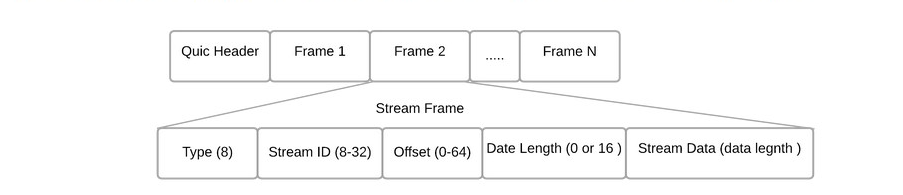
\includegraphics[width=1\columnwidth]{descrizione/quic/packet}
    \caption{\emph{QUIC Packet}}
    \label{quic-packet}
\end{figure}
\\
Gli \emph{header} si distinguono in due categorie, \emph{long header} e \emph{short header}. 
\\\\
Il \emph{long header} viene utilizzato principalmente durante l'inizializzazione della connessione. Contiene più informazioni ed è più dettagliato rispetto al \emph{short header}. Segue ora una breve descrizione dei campi presenti (Figura \ref{long-header}) \cite{site:Long-header}.
\begin{figure}[!h]
    \centering
    \begin{minipage}{0.48\textwidth}
        \centering
        \begin{small}
        \begin{BVerbatim}
 Long Header Packet {
   Header Form (1) = 1,
   Fixed Bit (1) = 1,
   Long Packet Type (2),
   Type-Specific Bits (4),
   Version (32),
   Destination Connection ID Length (8),
   Destination Connection ID (0..160),
   Source Connection ID Length (8),
   Source Connection ID (0..160),
   Type-Specific Payload (..),
 }
        \end{BVerbatim}
    \end{small}
        \caption{\emph{QUIC Long header}}
        \label{long-header}
    \end{minipage}
    \hfill
    \begin{minipage}{0.48\textwidth}
        \centering
        \begin{tabular}{|c|c|c|}
            \hline
            \textbf{Type} & \textbf{Name}  \\
            \hline
            0x00 & \emph{Initial} \\
            \hline
            0x01 & \emph{0-RTT}  \\
            \hline
            0x02 & \emph{Handshake}   \\
            \hline
            0x03 & \emph{Retry}  \\
            \hline
            \end{tabular}
        \caption{\emph{QUIC Long Header Packet Types}}
        \label{packet-type}
    \end{minipage}
\end{figure}

\begin{itemize}
    \item \textit{\textbf{Header Form}}: 1 bit, indica il tipo di \emph{header}, dove 1 indica \emph{long header}.
    \item \textit{\textbf{Fixed Bit}}: 1 bit, il valore fissato è 1 a meno che non sia un pacchetto di \emph{Negoziazione di Versione}. I pacchetti che contengono 0 in questo campo devono venire scartati.
    \item \textit{\textbf{Long Packet Type}}: 2 bit, specifica il tipo di pacchetto. I tipi di pacchetti sono specificati nella Figura \ref{packet-type}
    \item \textit{\textbf{Type-Specific Bits}}: 4 bit, contiene bit specifici per il tipo di pacchetto.
    \item \textit{\textbf{Version}}: 32 bit, indica la versione di \emph{QUIC} in uso.
    \item \textit{\textbf{Destination Connection ID Length}}: 8 bit, indica la lunghezza del \emph{Connection ID} di destinazione.
    \item \textit{\textbf{Destination Connection ID}}: 0 a 160 bit, indica il \emph{Connection ID} di destinazione.
    \item \textit{\textbf{Source Connection ID Length}}: 8 bit, indica la lunghezza del \emph{Connection ID} di origine.
    \item \textit{\textbf{Source Connection ID}}: 0 a 160 bit, indica il \emph{Connection ID} di origine.
    \item \textit{\textbf{Type-Specific Payload}}: lunghezza variabile, contiene il payload specifico per il tipo di pacchetto.
\end{itemize}

\noindent Una discussione approfondità sui singoli tipi di pacchetto in Figura \ref{packet-type} sarebbe troppo onerosa e non inerente. Pertanto vedremo velocemente il ruolo di ogni tipo senza entrare nel dettaglio. 
\\
\indent \textbf{\emph{Initial Packet}} ha il compito di trasportare il primo \emph{Crypto Frame} mandato dal \emph{client} e dal \emph{server} per fare lo scambio delle chiavi di crittografia, e si occupa anche di trasporta l'\emph{acknowledge} in entrambe le direzioni.
\\
\indent \textbf{\emph{0-RTT}}  ha il compito di trasportare gli \emph{early data} (dati anticipati) che il \emph{client} invia al \emph{server} come parte della prima comunicazione, questo permette di ridurre la latenza. Vedremo meglio questo nella sezione dedicata all'\emph{handshake}.
\\
\indent \textbf{\emph{Handshake Packet}}  ha il compito di trasportare i messaggi crittografici necessari per il processo di handshake. Una volta che il \emph{client} ha ricevuto un \emph{Handshake packet} dal \emph{server}, , il \emph{client} utilizza pacchetti di \emph{handshake} per inviare i successivi messaggi criptografici di \emph{handshake} e riconoscimenti al \emph{server}.
\\
\indent \textbf{\emph{Retry Packet}}  ha il compito di trasportare un \emph{token} di validazione creato dal \emph{server}. Viene usato dal \emph{server} quando vuole effettuare un \emph{retry}, ovvero richiedere al \emph{client} di ripetere l'invio di una richiesta iniziale.
\\\\
Passiamo ora ad analizzare il \emph{short header}, utilizzato esclusivamente dopo che le chiavi sono state negoziate. Esiste un'unica variante di questo \emph{header}, noto come RTT-1 (illustrato nella Figura \ref{short-header}) \cite{site:Short-header}.
\begin{figure}[!h]
    \centering
    \begin{small}
    \begin{BVerbatim}
1-RTT Packet {
    Header Form (1) = 0,
    Fixed Bit (1) = 1,
    Spin Bit (1),
    Reserved Bits (2),
    Key Phase (1),
    Packet Number Length (2),
    Destination Connection ID (0..160),
    Packet Number (8..32),
    Packet Payload (8..),
  }
    \end{BVerbatim}
\end{small}
    \caption{\emph{QUIC Short header}}
    \label{short-header}
\end{figure}
\begin{itemize}
    \item \textit{\textbf{Header Form}}: 1 bit, indica il tipo di \emph{header}, dove 0 indica \emph{short header}.
    \item \textit{\textbf{Fixed Bit}}: 1 bit, il valore fissato è 1. I pacchetti che contengono 0 in questo campo devono venire scartati.
    \item \textit{\textbf{Spin Bit}}: 1 bit, viene utilizzato per il monitoraggio passivo della latenza, il \emph{server} riflette il valore dello \emph{spin bit} ricevuto mentre il \emph{client} lo inverte dopo ogni \emph{RTT}.
    \item \textit{\textbf{Reserved Bits}}: 2 bit, sono dei bit riservati e protetti usando l'\emph{header protection}, il loro valore dopo aver rimosso la protezione deve essere 0, in caso contrario viene segnalato un errore di connessione.
    \item \textit{\textbf{Key Phase}}: 1 bit, indica la fase della chiave, ovvero permette a chi riceve il pacchetto di identificare le chiavi usate per proteggere il pacchetto. Anche questo campo è protetto usando l'\emph{header protection}.
    \item \textit{\textbf{Packet Number Lenght}}: 2 bit, indica la lunghezza effettiva del campo \emph{Packer Number}
    \item \textit{\textbf{Destination Connection ID}}: 0 a 160 bit, indica il \emph{Connection ID} scelto da chi riceve il pacchetto.
    \item \textit{\textbf{Packet Number}}: 8 a 32 bit, contiene il \emph{Packet Number}.
    \item \textit{\textbf{Packet Payload}}: 8 a lunghezza variabile, contiene il \emph{payload} protetto. 
    \end{itemize}
\subsubsection{Handshake}
Qui si parla del processo di handshake
domani 
\subsubsection{Multiplexing}
Qui si parla del processo di handshake
domani 
\subsubsection{Gestione degli Errori e di Ritrasmissione}

Qui si parla della gestione degli Errori e di ritrasmissione

\subsubsection{Sicurezza del Protocollo}

Gestione del lato di sicurezza del protocollo
1 intero giorno 

\subsubsection{Versione e Applicazioni }
% https://quicwg.org/
Dove viene usato, versioni e tecnologie etc.

\subsection{MPTCP}

Qua c'è molto da
Da pensare ai capitoli 

\section{I problemi e l'Idea}

I problemi di Quic e le nostre idee.


